\def\layersep{2.5cm}

\begin{figure}[H]
\center
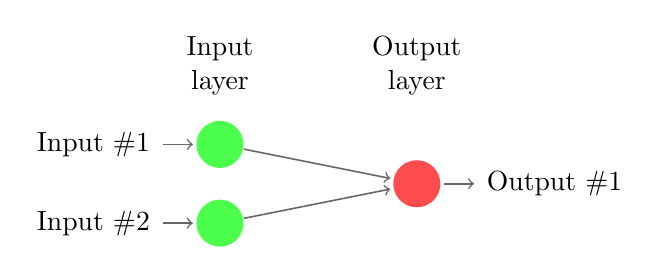
\begin{tikzpicture}[shorten >=1pt,->,line width=0.2mm,draw=black!60, node distance=\layersep]
    \tikzstyle{every pin edge}=[<-,shorten <=1pt]
    \tikzstyle{neuron}=[circle,fill=black!25,minimum size=17pt,inner sep=0pt]
    \tikzstyle{input neuron}=[neuron, fill=green!70];
    \tikzstyle{output neuron}=[neuron, fill=red!70];
    \tikzstyle{hidden neuron}=[neuron, fill=blue!70];
    \tikzstyle{annot} = [text width=4em, text centered]

    % Draw the input layer nodes
    \node[input neuron, pin=left:Input \#1] (I-1) at (0,-1) {};
    \node[input neuron, pin=left:Input \#2] (I-2) at (0,-2) {};

    % Draw the output layer node
    \node[output neuron,pin={[pin edge={->}]right:Output \#1}] (O-1) at (\layersep,-1.5) {};

    % Connect every node in the input layer with every node in the
    % hidden layer.
    \path (I-1) edge (O-1);
    \path (I-2) edge (O-1);

    % Annotate the layers
    \node[annot,above of=I-1, node distance=1cm] (il) {Input layer};
    \node[annot,right of=il] {Output layer};
\end{tikzpicture}
\caption{Perceptron with two inputs and one output. \label{fig:perceptron}}
\end{figure}